\documentclass[11pt,a4paper,spanish,twocolumn]{article}
\usepackage{estilo_unir_articulo}
\usepackage{standalone}
\usepackage{subcaption} % conflicto con subfig
% diagramas simples
\usepackage{tikz}
\usepackage{pgfplots}
\pgfplotsset{compat=1.16}
\usetikzlibrary{shapes.geometric, arrows}
\usepackage{tikz-uml}
\tikzumlset{fill class=white!20, fill template=white!15,font=\bfseries\footnotesize}

%%% Definiciones para diagramas flowchart
\tikzstyle{startstop} = [rectangle, rounded corners, minimum width=3cm, minimum height=1cm,text centered, draw=black, fill=red!30]
\tikzstyle{io} = [trapezium, trapezium left angle=70, trapezium right angle=110, minimum width=2cm, minimum height=1cm, text centered, draw=black, fill=blue!30]
\tikzstyle{process} = [rectangle, minimum width=3cm, minimum height=1cm, text centered, draw=black, fill=orange!30]
\tikzstyle{decision} = [diamond, minimum width=3cm, minimum height=1cm, text centered, draw=black, fill=green!30]
\tikzstyle{arrow} = [thick,->,>=stealth]

\usepackage{tabularx}
\usepackage[flushleft]{threeparttable}
\usepackage{multirow}

\usepackage{ifthen}
\newcommand\pincludegraphics[2][0.98]{
  \def\scale{#1}
  \def\graphname{img/#2}
  \def\texfigure{img/#2.tex}
  \def\pgffigure{img/#2.pgf}
  \IfFileExists{\texfigure}{
    \resizebox{\scale\columnwidth}{!}{
      \includestandalone{\graphname}
    }
    }{
    \IfFileExists{\pgffigure}{
      \resizebox{\scale\columnwidth}{!}{
        \input{\pgffigure}
        %\includestandalone{\pgffigure}
        %\includegraphics[width=\scale\columnwidth]{\pgffigure}
      }
      }{
      % \includegraphics[scale=\scale\columnwidth]{\graphname}
      \includegraphics[width=\scale\linewidth]{\graphname}
    }
  }
}

\def\accelcapture/{\textsl{\textsf{Accel}}\textsf{Capture}}
\def\ifell/{\textsl{\textsf{i}}\textsf{Fell}}
\def\g/{~\textsl{g}}


\newcommand\tablan[7][\columnwidth]{
  \def\myscale{#1}
  \def\mytableid{#2}
  \def\mycaptiontext{#3}
  \def\mycolumnstyles{#4}
  \def\mytablecontent{#5}
  \def\tablenote{#6}

  \begin{table}
    \caption{\label{\mytableid} \mycaptiontext}
    % \rowcolors{#7}{white}{Gray!20}
    \centering
    \resizebox{\myscale}{!}{
    % \scalebox{0.5}{
      \begin{threeparttable}
        \begin{tabular}{@{}#4@{}}
          \toprule[1.5pt]
          #5
          \bottomrule[1.5pt]
        \end{tabular}

        \begin{tablenotes}
          \small
          #6
        \end{tablenotes}
      \end{threeparttable}
    }
  \end{table}
}


% para usar \currenttime
\usepackage{datetime}

% mejores tablas, midrule, toprule, bottomrule
\usepackage{booktabs}

%---------------------------
%título del trabajo y autor
%---------------------------
\title{Detección de caídas en dispositivos vestibles con RNN}
\author{Aritz Beraza Garayalde}
\date{\today}


%---------------------------
%marges
%---------------------------
%\usepackage[margin=1.9cm]{geometry}
%---------------------------
%---------------------------
%---------------------------
%---------------------------

\resumen{En sociedades cada vez más envejecidas aumenta la necesidad de controlar de forma continua la salud de las personas mayores. En especial de identificar las caídas, una de las principales causas de mortalidad en personas mayores. Existen soluciones que sirven a este propósito, pero son sistemas específicos, basados en unidades de cómputo externas, caros, obtrusivos y que restringen la libertad de acción del usuario. Este trabajo se presenta un sistema de detección de caídas que funciona de forma autónoma en un reloj inteligente o \textit{smartwatch} integrando en un mismo dispositivo las capacidades de captura, detección y alerta en. Usando un algoritmo híbrido para mejorar la autonomía y un novedoso sistema de detección de anomalías basado en la arquitectura codificador/decodificador implementamos un sistema que mejora notablemente las capacidades de los métodos analíticos y se acerca a la exactitud del estado del arte en sistemas de detección mediante inteligencia artificial.}
\palabrasclave{Detección de caídas, algoritmo híbrido, GRU, codificador/decodificador}


\begin{document}
\twocolumn[
\begin{@twocolumnfalse}
\maketitle
\end{@twocolumnfalse}
]

%\renewcommand{\listfigurename}{Índice de Ilustraciones}
%\renewcommand{\listtablename}{Índice de Tablas}
%\renewcommand{\contentsname}{Índice de Contenidos}
%\renewcommand{\figurename}{Figura}
%\renewcommand{\tablename}{Tabla} 
%\twocolumn


%\frontmatter
%\tableofcontents
%\listoffigures
%\listoftables

\section{INTRODUCCIÓN}
La población de las sociedades occidentales envejece rápidamente a consecuencia de la mengua en la tasa de fertilidad y al incremento en la esperanza de vida. Así, la Organización Mundial de la Salud  informa que los adultos mayores de 65 años tienen un mayor riesgo de sufrir caídas y recomienda priorizar la investigación para mejorar la atención médica en estos casos \cite{FactsFalls2018}.
Gracias a los avances en miniaturización de sensores desde hace años existen sistemas basados en la interpretación analítica de lecturas de la aceleración y posición del cuerpo para identificar la actividad física llevada a cabo\cite{fallindex00,Chen2005,Bourke2006}, considerando las caídas como una actividad o familia de actividades más. En los últimos años, y gracias a la mejora en la capacidad de cálculo de los microprocesadores aparecen modelos basados en técnicas de aprendizaje automático para realizar estas clasificaciones\cite{Noury2007, Ozdemir2014} mejorando notablemente la exactitud a la hora de detectar las caídas a costa de un incremento en las necesidades de capacidad de cálculo, resultando sistemas que requieren una conexión con una unidad de procesado externo\cite{Yang2010} o en sistemas con autonomías de funcionamiento reducidas que no llegan a completar un día de funcionamiento\cite{Liu2020}.

Los dispositivos llevables (del inglés \emph{wearables}, dispositivos electrónicos compuestos por sensores y microprocesadores que se incorporan en alguna parte del cuerpo) y portables han proliferado en la sociedad hasta ser omnipresentes. Ya sea mediante un teléfono móvil\cite{tfall} o combinando una pulsera de actividad o similar y una dispositivo móvil\cite{Vilarinho2015} han ido apareciendo soluciones para implementar sistemas de detección de caídas que simplifican su utilización. Sin embargo ninguno se adecua a las personas mayores. Este grupo de población carece de los conocimientos necesarios para manipular sistemas electrónicos e incluso muchas veces los rehuyen.

Con el objetivo de eliminar esta barrera y acercar a las personas mayores un sistema de detección de caídas que se adapte a sus necesidades y capacidades, autónomo y con la potencia de los modelos basados en aprendizaje automático, presentamos un desarrollo que aunando en un algoritmo híbrido un modelo analítico eficiente en recursos y otro basado en redes neuronales recurrentes permita obtener un sistema de alta capacidad de detección de caídas y autonomía en un formato compacto, funcional y sencillo como es un reloj de pulsera. Mediante técnicas de aprendizaje no supervisado y gracias a una base de datos de entrenamiento generada para el sistema obtendremos un modelo de detección de anomalías mediante comparación de la raíz del error cuadrático medio de una red neuronal recurrente con arquitectura codificador/decodificador. Este sistema, activado por un modelo analítico de baja complejidad a modo de generador de eventos, permite obtener un sistema de detección y alerta de caídas completamente funcional con una autonomía que puede alcanzar varios días y que permite alertar de forma local y remota mediante notificaciones a un servidor por Internet.


\section{ESTADO DEL ARTE}
Los primeros sistemas de teledetección de caídas aparecen a finales del siglo pasado\cite{Williams1998}, gracias al desarrollo de las telecomunicaciones y sistemas embebidos usando modelos de análisis de la aceleración y posición del cuerpo. Posteriores estudios ofrecen mejoras en los algoritmos añadiendo etapas de detección y confirmación de la caída\cite{Chen2005,Bourke2008}, y en la miniaturización de las unidades de cómputo hasta hacerlas llevables\cite{fallindex00}. Estos modelos sin embargo adolecen de grandes limitaciones en sus capacidades de detección ya que los resultados obtenidos se calculan con bases de datos adaptadas al experimento en cuestión y se comportan peor de lo esperado en pruebas reales\cite{Bagala2012}, sin embargo la creciente potencia de los microprocesadores facilita su implementación en sistemas embebidos. Los modelos y algoritmos de detección basados en  inteligencia artificial o aprendizaje automático empiezan a aplicarse al problema de la detección de actividades humanas\cite{Noury2007,Ozdemir2014} demostrando su superioridad y mayor capacidad para generalizar el aprendizaje y realizar detecciones en uso real\cite{Aziz2017}. Estos métodos por contra requieren de potentes sistemas de cálculo con unidades de paralelización de calculo y por tanto volvemos a los sistemas compuestos por unidades de captura y de procesado por separado\cite{Ajerla2019} o adolecer de autonomías que no cubren un día completo de uso\cite{Liu2020}.

En cuanto a los modelos usados, prácticamente cualquier sistema de clasificación o segmentación: Bayes, k-NN, CNN, RNN, Árboles de decisión, SVM, etc.\cite{Liu2018,Anita2020}. Sin embargo es un terreno en el que aparecen cada día nuevas opciones como es aplicar RNN Codificador/Decodificador aplicada con éxito al procesado del lenguaje\cite{Cho2014,Serban2017} para realizar detección o predicción de anomalías mediante señales temporales\cite{Park2018,Peng2018}. 

Las técnicas de optimización de modelos basados en redes neuronales inician su andadura al proponer eliminar pesos de menor importancia y entrenar la red restante para sobreponer el daño ocasionado\cite{RNN1986} de forma similar a como hace un cerebro animal. Combinado con técnicas de reducción de la precisión de los pesos se consigue reducir el tamaño, a menos de una cuarta parte y multiplicar el rendimiento con impactos mínimos en la calidad de los modelos y mejorando su eficiencia\cite{han2015,Guo2018,Jin2019}. Otros acercamientos proponen el uso de algoritmos híbridos para reducir el consumo mediante la combinación de un modelo analítico que actúe como filtro o generador de eventos para la activación de un segundo modelo con mayor consumo de recursos\cite{Lim2014, Putra2017} aunando eficiencia y capacidad de detección.

\section{OBJETIVOS Y METODOLOGÍA}
Con este trabajo abordamos la implementación de un sistema de detección de caídas llevable, autónomo e independiente que aúne en una unidad la captura de datos y la detección de caídas que a su vez esté orientado al uso por parte de personas mayores con edades superiores a 65 años.

\subsection{Bases de datos de actividad}
El número de bases de datos de actividad humana y caídas disponible públicamente es muy reducido \cite{igual2015} y la mayoría están orientados al experimento para el que fueron creadas. De todos,  UMAFall\cite{Edu/UMA/2017} es el único que se ajusta a este trabajo por contener capturas desde la muñeca. Sin embargo no está lo suficientemente extendido para realizar una evaluación comparativa. Optamos por generar un conjunto de datos propio para el entrenamiento y usar SisFall\cite{Sucerquia2017} para definir los umbrales de decisión y validar el algoritmo y modelos. SisFall está especialmente orientada a la detección de caídas con 4504 eventos de los cuales 1798 pertenecen a caídas, grabados por 38 participantes, de los cuales 23 con edades comprendidas entre los 60 y 75 años, ajustándose a los requisitos de este trabajo. Incluye información de la aceleración capturada desde la cintura, así que en debemos validar que hay una correlación entre los valores de la aceleración capturados en muñeca y cintura para poder combinar ambos resultados.

Para generar la base de datos de actividad \accelcapture/ usamos reloj inteligente Fossil Sport Gen 3 (\ref{tab:watch:specs}), la misma plataforma sobre la que realizaremos el desarrollo final. Este dispositivo contiene un sensor triaxial para medir la aceleración, siendo capaz de leer a 50 muestras por segundo. Mediante una aplicación desarrollada para la ocasión: \accelcapture/.

\begin{table}\caption{\label{tab:watch:specs} Especificaciones de la plataforma Fossil Sport Gen 3 reportadas por el Sistema Operativo}
	\begin{tabular}{lc}\toprule
  \emph{Nombre}              & Fossil Gen3 Sport \\
\emph{Tamaño Pantalla}     & 1,4" \\
\emph{Formato}              & Circular \\
\emph{Tipo de Pantalla}    & Táctil color (AMOLED) \\
\emph{Resolución}          & 454 x 454 px \\
\emph{Bluetooth}           & 4.1 \\
\emph{Wifi}                & 802.11 b/g/n \\
\emph{ROM}                 & 4GBytes \\
\emph{RAM}                 & 512MBytes \\
\emph{CPU}                 & Snapdragon 2100 \\
\emph{OS}                  & WearOS 2 \\
\emph{Sensor Freq. Cardiaca} & Si \\
\emph{Giroscopio}          & Si \\
\emph{Acelerómetro}         & 3 ejes \\
\emph{~~Frecuencia}         & 50\hz/ \\
\emph{~~Resolución}					& 0,00119 $m/s^2$ \\
\emph{~~Valor Máximo}				& 384,8867 $m/s^2$\\ \bottomrule
\end{tabular}
\end{table}

La aplicación creada para leer las sesiones de actividad (apodada \emph{AccelCapture}) usa un comparador para detectar actividad cuando el índice $\Delta \vec{A}_n = |\|\vec{A}_n\| -\|\vec{A }_{n-1}\||$ supera ya sea un índice de actividad instantánea de 2\g/ o durante una ventana de 5 segundo el promedio es superior a 0,3\g/.

\begin{figure}
  \pincludegraphics{capturaFlujo}
  \caption{\label{fig:accelcapture:flow} Diagrama de flujo de la aplicación \accelcapture/}
\end{figure}

Finalmente se conforma una base de datos con presencia únicamente de secuencias de los tres ejes de la aceleración sin presencia de caída alguna, únicamente actividades cotidianas o situaciones que a pesar de encontrarse el sujeto estacionario se ejerza sobre el una aceleración, como pueda ser viajar en un medio de transporte como un coche o un avión. La base de datos dispone de 37563 segundos de capturas de actividad en 274 sesiones diferentes realizadas por 3 sujetos de edades que oscilan entre los 34 y 77 años llevando el dispositivo en la muñeca izquierda, siendo esta su mano no predominante. 

\begin{table}
  \caption{\label{tab:accelcapture:description} Resumen de características de la base de datos}
  \begin{tabular}{lc}\toprule
  \textit{Atributo}      & \textit{Valor}  \\\midrule
  Sesiones      & 274    \\
  Sujetos       & 3      \\
  Sensor        & Acel. 3 ejes \\
  Frecuencia Muestreo & 50\hz/  \\
  Unidades medida & $m/s^2$  \\ \bottomrule
  \end{tabular}
\end{table}

Finalmente de cara al entrenamiento y validación debemos submuestrear ambos conjuntos. Para reducir el consumo, el reloj muestreará a únicamente 25\hz/ que es suficiente para permitir realizar la detección de actividades\cite{Liu2018}, por lo que será necesario reducir el número de lecturas de las basos de datos: para Sisfall, capturada a 200\hz/ mantendremos una de cada 8 muestras mientras que para \accelcapture/ tomaremos muestras alternas. Este proceso lo realizamos tras filtrar con un filtro IIR paso bajo de primer orden ($H(z) = \frac{\alpha}{1-(1-\alpha)z^{-1}}$) con frecuencia de corte a 12,5\hz/ ya que es el máximo ancho de banda permitido por Nyquist. 

\begin{figure}
  \pincludegraphics{capturaFlujo}
  \caption{\label{fig:accelcapture:flow} Diagrama de flujo de la aplicación \accelcapture/}
\end{figure}

Para comprobar la similitud entre las distribuciones de la aceleración de ambos conjuntos analizamos los histogramas de valores de pico en la figura \ref{fig:accelcapture:hitogram}. Finalmente separamos de SisFall dos conjuntos: el 80\% de las muestras en el conjunto de entrenamiento  y un 20\% para el de validación ($SF_{test}$ y $SF_{val}$ respectivamente). A su vez de ambos grupos extraemos el subconjunto de eventos de actividad ($SFA_{test}$ y  $SFA_{val}$) que serán usados para calcular los umbrales de decisión finales. 
\begin{figure}
  \centering
  \begin{subfigure}[b]{0.49\columnwidth}
      \centering
      \pincludegraphics{AccData_histoLow}
      \caption{\footnotesize Valores valle SisFall y \accelcapture/}
      \label{fig:accelcapture:hitogram:low}
  \end{subfigure}
  \hfill
  \begin{subfigure}[b]{0.49\columnwidth}
      \centering
      \pincludegraphics{AccData_histoUp}
      \caption{\footnotesize Valores pico SisFall y \accelcapture/}
      \label{fig:accelcapture:hitogram:high}
  \end{subfigure}
  \caption{\label{fig:accelcapture:hitogram} Histogramas de valores pico y valle}
\end{figure}


\subsection{Generación de modelos}
Nuestro desarrollo hace uso de dos modelos, uno analítico y otro basado en redes neuronales recurrentes. El modelo analítico elegido es Bourke \cite{Bourke2006}. Un modelo que por construcción garantiza el 100\% de sensibilidad sobre el conjunto de datos elegido y que de acuerdo con las limitaciones de nuestro sistema, no requiere de información de la posición del individuo ni del sensor pues procesa únicamente el vector suma de la aceleración (la norma del mismo): $SVA = \|\vec{A}\|=\sqrt{A_x^2 + A_y^2 + A_z^2}$. 

\subsubsection{Modelo de Bourke}
Para configurar el modelo de Bourke realizamos un análisis de los valor pico y valle de la aceleración en cada instancia del conjunto $SF_{test}$. Tal y como define el algoritmo definiremos una cota superior establecida de manera que todas las muestras de caídas tengan un pico que supere dicho valor y a la inversa con el valor de valle, asegurando que toda caída tiene un valor de valle inferior. Para este ejercicio usaremos un comparador \textit{Bourke U} que únicamente mira que se supere el umbral de pico ya que es el que mejor capacidad de segregar caídas de actividad dispone. Analizando los percentiles de la distribución de valores máximo de la aceleración en una caída obtenemos un valor de cota de 4,16\g/ y una especificidad del 22\% que crece rápidamente si aceptamos reducir ligeramente la sensibilidad tal y como se observa en la tabla \ref{tab:umbrales}.

\begin{figure}
  \pincludegraphics{BourkeThresholds}
  \caption{\label{fig:bourke:thresholds} Cotas pico y valle de Bourke}
\end{figure}

\subsubsection{Modelos RNN}
Generaremos varios modelos para analizar el impacto de la estructura de la red y tamaño de las celdas GRU usadas en el estimador obtenido. Principalmente generaremos dos familias de de modelos: los modelos basados en la predicción de la caída y los modelos que realizarán una reconstrucción de la misma. En el fondo son estructuras casi idénticas pero que han sido entrenadas para obtener resultados diferentes. Partiendo de la secuencia de datos de la aceleración, calculamos la norma en cada instante a partir de sus componentes y generamos dos ventanas: $W^{in} = $ y $W^{out}$ que se corresponden con el valor de entrada y el valor esperado de salida del modelo a entrenar: $X = W^{in}, Y=W^{out}$.

\paragraph{Modelos RNN-Reconstrucción}
La señal de entrada y la esperada de salida son las mismas: $X=Y=W^{in}=^{out}$. De longitud 100 muestras ambas.
\paragraph{Modelos RNN-Predicción}
La señal de entrada y salida son una la continuación de la otra, y además de diferente tamaño. $W^{in}$ mantiene las 100 muestras mientras que $W^{out}$ se reduce a 50. Lo denominamos de predicción por que la secuencia contenida en $W^{out}$ es la continuación de la señal de entrada: $W^{in} =[x_0, x_1,\cdots,x_{99}]$ y $W^{out}=[x_100, x_101, \cdots,x_149]$.

\begin{figure}
  \pincludegraphics{Prediction_reconstruction}
  \caption{\label{fig:ifell:reconstrucion} Predicción de la aceleración por un modelo RNN Codificador/Decodificador}
\end{figure}

Generamos los modelos usando TensorFlow y los entrenaremos durante un máximo de 250 épocas con un sistema de parada temprana y tasa de aprendizaje decreciente de forma polinómica, con incrementos relativos menores al principio para acelerar el aprendizaje y mayores al final para conseguir un ajuste fino de los mismos. En este punto apreciamos una clara tendencia alsobreajuste de los modelos basados en la predicción como se aprecia en la figura \ref{fig:rnn:predict:train}.

\begin{figure}
  \centering
  \begin{subfigure}[t]{0.49\columnwidth}
    \centering

    \pincludegraphics{trainingModeloRNNPred350-25}
    \caption{\label{fig:rnn:predict:train} RMSE en entrenamiento de un modelo de predicción}
  \end{subfigure}
  \hfill
  \begin{subfigure}[t]{0.49\columnwidth}
    \centering
    \pincludegraphics{trainingModeloRNNRecon350-50}
    \caption{\label{fig:rnn:reconstrucion:train} RMSE en entrenamiento de un modelo de reconstrucción}
  \end{subfigure}
  \caption{\label{fig:rnn:train} Función de pérdida durante el entrenamiento de los modelos}
\end{figure}

Haremos dos tipos de experimentos con estos modelos. Entrenarlos y validarlos con SisFall, mediantes los conjuntos $SF_{test}$ y $SF_{val}$ y entrenarlos con \accelcapture/ y validarlos con SisFall. Denominaremos a estos modelos $RNN\_<tipo>(<uds>)[<atr>]$ y a los modelos entrenados con SisFall y $IFALL\_<tipo>(<uds>)[<atr>]$ los modelos entrenados con \accelcapture/, donde \textit{<tipo>} puede ser "P" para predicción y "R" para reconstrucción, \textit{<uds>} son las unidades de las celdas y \textit{<atr>} el número de atributos del espacio intermedio.

Una vez confirmada la validez del modelo, aplicaremos diferentes técnicas de optimización y reducción de modelos neuronales para lograr un menos consumo de memoria y recursos y adaptarlo a la plataforma elegida reduciendo la latencia y consumo con el fin de lograr un sistema con autonomía suficiente para más de un día de uso, con el fin de lograr un símil entre el recargar la plataforma presentada y el remontuar un reloj mecánico con el que el público objetivo estaría familiarizado y lograr por tanto realizarlo a intervalos similares.

Finalmente implementaremos una aplicación para el sistema orientada siempre a la facilidad de uso intentando mantener las mismas sinergias de sus homólogos mecánicos y en última instancia evaluaremos el grado de satisfacción con el sistema logrado tras dos meses de uso.

\section{CONTRIBUCIÓN}
Este trabajo presenta por primera vez un sistema híbrido con una etapa analítica simple y un modelo de redes neuronales recurrentes corriendo sobre un sistema llevable manteniendo una autonomía superior a las 24 horas de uso continuo de forma consistente. Así mismo aplica la arquitectura RNN Codificador/decodificador por primera vez a la detección de anomalías en la actividad humana permitiendo detectar caídas como anomalías usando entrenamiento no supervisado.


\subsection{Modelo híbrido}

Proponemos el modelo con dos etapas definido por el diagrama de la figura \ref{fig:ifell:algorithm}. La primera etapa basada en un modelo analítico \textit{BourkeU}. Este modelo funciona como un filtro o generador de eventos. Se encarga de dejar pasar únicamente los eventos mejores candidatos a caídas. Una vez detectada la caída en un un instante $t_0$, conforma las ventanas $W^{in}$ y $W^{out}$ que enviar al modelo RNN posterior. Estas ventanas cambian según el tipo de modelo:
\begin{itemize}
  \item \textit{Predicción} $W^{in} = [x_{t_0 - 125},\cdots, x_{t_0-25}]$ y $W^{out}=[x_{t_0-24},\cdots,x_{t_0},\cdots,x_{t_0+50}]$
  \item \textit{Reconstrucción} $W^{in} = W^{out} = [x_{t_0-49},\cdots,x_{t_0},\cdots,x_{t_0+50}]$
\end{itemize}

\begin{figure}
  \centering
  \pincludegraphics[0.6]{deteccionFlujo}
  \caption{\label{fig:ifell:algorithm} Diagrama del algoritmo híbrido de \ifell/}
\end{figure}

Estas ventanas se entregan al modelo RNN Codificador/Decodificador que es el encargado de procesarlas y mediante la comparación del error RMSE entre la salida generada y la esperada decide si se ha producido una anomalía o caída.


\subsubsection{RNN Codificador/Decodificador}
Proponemos por primera vez un sistema codificador/decodificador RNN para detectar caídas como anomalías en la actividad cotidiana. Esta arquitectura realiza una primera extracción de características mediante una red neuronal recurrente y posteriormente mediante una segunda red recurrente alimentada por este vector de características realizar bien una predicción bien una reconstrucción de la señal original. Comparando el error cometido en la reconstrucción o en la señal predicha podemos establecer un umbral de decisión entre actividad ordinaria o anomalía (entre las que se incluirian las caídas). 

\begin{figure}
  \pincludegraphics{modeloRNNarticulo}
  \caption{\label{fig:ifell:archi} Arquitectura de la red RNN Codficador/Decodificador Reconstrucción \ifell/}
\end{figure}

Entrenamos variaciones de modelos tanto de reconstrucción como de predicción de señal variando el tamaño de las celdas GRU como el número de atributos obtenidos por el codificador para estudiar el tamaño óptimo de la red que maximice la capacidad de detección manteniendo unos tiempos de ejecución por debajo del segundo en el reloj.

\subsection{Implementación de la aplicación}

\paragraph{Optimización de los modelos}
Los modelos obtenido no pueden ser usados directamente. Es necesario convertirlos a TensorFlow Lite, para el que existe un intérprete compatible con el dispositivo usado. Además, para maximizar el rendimiento aplicamos pruning para obtener un modelo ralo: Eliminar el 50\% de los pesos de la red de forma progresiva. Este proceso se puede entender como una normalización similar a la técnica de \textit{Dropout} con la salvedad de que la eliminación de nodos no se realiza de forma aleatoria sino por su aportación a la respuesta final y por que esta eliminación es definitiva. Bien configurado los efectos son similares pues mediante entrenamiento adicional la red resultante puede llegar a mejorar la capacidad de generalización del modelo original\cite{Cai2020}, aunque en nuestras muestras la mayoría de los casos ha resultado en una ligera pérdida de calidad de los modelos.

El modelo ralo resultante es cuantizado para reducir todavía más su tamaño según la tabla \ref{tab:model:optim}. Cuantizar reduce la precisión de la representación de los pesos de la red. Además, en la conversión a enteros se consigue mejorar el rendimiento en sistemas sin unidades de cálculo de coma flotante. Nuestro caso las latencias de los modelos GRU de 175 unidades y 50 atributos se reducía de 2,611 segundos con cuantizado a coma flotante de 16 bits a 1,200 con conversión a enteros de 8 bits.

\begin{table}\caption{\label{tab:model:optim} Reducción del tamaño del modelo en MBytes con cada técnica de optmización}
  \resizebox{\columnwidth}{!}{
    \begin{tabular}{lccc}\toprule
      \emph{Modelo}       & \emph{Orig.}  & \emph{C. Enteros}  & \emph{C. Float16} \\ \midrule
      RNN-(350)[50]            & 15,2          & 4,0                   & 7,7 \\
      RNN-(175)[50]            & 4,0           & 1,1                   & 2,0 \\ \bottomrule
    \end{tabular}
  }
\end{table}

\paragraph{Aplicación \ifell/}

\ifell/, la aplicación resultante de este trabajo es un armazón en torno al algoritmo y modelos ya definidos encargado de proveer de datos a los mismos y de reaccionar a los eventos de detección de caída generando una alarma (que activa una respuesta visual, háptica y acústica en el dispositivo mismo y envía una notificación con detalles del evento a un servidor en internet para notificar a terceras personas que puedan ofrecer asistencia.

\begin{figure}[!ht]
  \centering
  \begin{subfigure}[b]{0.48\columnwidth}
      \centering
      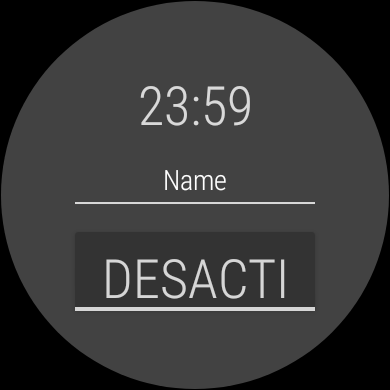
\includegraphics[width=\linewidth]{img/appActivity.png}
      \caption{\footnotesize Aplicación de gestión}
      \label{fig:uiActivity}
  \end{subfigure}
  \hfill
  \begin{subfigure}[b]{0.48\columnwidth}
      \centering
      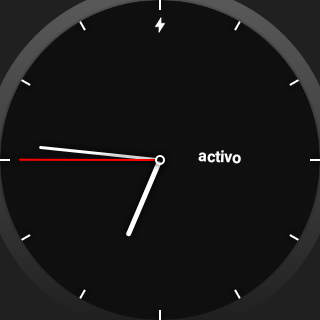
\includegraphics[width=\linewidth]{img/appWatchface.png}
      \caption{\footnotesize Interfaz esfera de reloj}
      \label{fig:uiWatchface}
  \end{subfigure}
  \begin{subfigure}[b]{0.48\columnwidth}
      \centering
      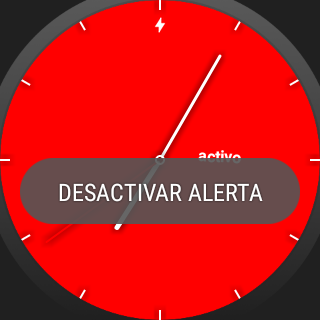
\includegraphics[width=\linewidth]{img/appAlerta.png}
      \caption{\footnotesize Pantalla de alerta de caída}
      \label{fig:uiAlerta}
  \end{subfigure}
  \hfill
  \begin{subfigure}[b]{0.48\columnwidth}
      \centering
      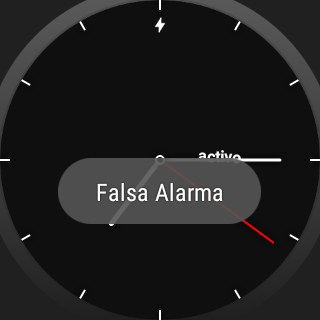
\includegraphics[width=\linewidth]{img/appAlertaFalsa.png}
      \caption{\footnotesize Pantalla en caso de predetección de caída}
      \label{fig:uiAlertaFalsa}
  \end{subfigure}
  \caption{\footnotesize \label{fig:ifell:UI} Interfaz de usuario de \ifell/}
\end{figure}

La aplicación toma el aspecto visual de una esfera de reloj analógica que a su vez se convierte en el sistema de alerta visual. La aplicación, una vez instalada no requiere de ninguna intreacción por parte del usuario. Al ser una esfera, el propio sistema operativo se encarga de lanzarla tras cada inicio del sistema así como de mantener su proceso activo y ejecutándose. A su vez la aplicación está formada por dos servicios asíncronos:
\begin{itemize}
  \item Captura y Alerta: Realiza la captura de datos del sensor. Implementa la primera fase del algoritmo: el modelo de Bourke.  Si este detecta una caída, prepara las ventanas de entrada y salida para alimentar al modelo RNN. A su vez, atiende las respuestas del modelo de detección para actuar en consecuencia.
  \item Procesado de las muestras. Implementa el modelo RNN propuesto. Es alimentado de forma asíncrona por el proceso anterior, de forma que puede permanecer en hibernación hasta ser requerido.
\end{itemize}

\section{RESULTADOS O EVALUACIÓN }

De cara a le evaluación final, generamos los mejores modelos candidato y los entrenamos con la base de datos \accelcapture/ durante un máximo de 250 épocas con un mecanismo de parada temprana si el error RMSE deja de descender durante 5 iteraciones seguidas. Posteriormente usaremos el subconjunto de test de SisFall para calcular los umbrales de decisión de Bourke y RMSE  validación que separamos previamente para estudiar las estadísticas del modelo. En la tabla \ref{tab:umbrales} se listan los umbrales de decisión según el percentil de caídas que dejan de detectar. Tomamos en este punto la decisión de sacrificar 0,6\% de sensibilidad del algoritmo de Bourke para mejorar su especificidad hasta el 30\%.

\begin{table}\caption{\label{tab:umbrales}Umbrales de decisión para Bourke y Modelos RNN}
  \resizebox{\columnwidth}{!}{
    \begin{tabular}{lcccc}\toprule
      \emph{Umbral}   & p.0\% & p.1\%  & p.3\%  & p.5\%  \\ \midrule
      Bourke Pico  & 4,16\g/ & 5,77\g/ & 6,67\g/ & 7,40 \g/ \\
      IFELL-P(175)[50] & 0,6956 & 1,6145 & 1,9264 & 2,2176  \\
      IFELL-R(175)[50] & 0,0701 & 0,1404 & 0,2358 & 0,2822 \\ \bottomrule
    \end{tabular}
  }
\end{table}

Al ser un clasificador usaremos para este fin las métricas:
\begin{itemize}
  \item Sensitividad (Capacidad de identificar las caídas), también conocida como \textit{recall}.
  \[
    Sensitividad = \frac{TP}{TP+FN}
  \]
  \item Especificidad o Selectividad (Capacidad de discernir únicamente las caídas).
  \[
    Especificidad = \frac{TN}{TN+FP}
  \]
\item Exactitud promediada (Sesgo de la clasificación, como de seguros podemos estar del resultado del clasificador)
  \[
  Exactitud~Prom.=\frac{Sens.+Esp.}{2}
  \]
\end{itemize}
Estas métricas son ampliamente utilizadas en los estudios relacionados \cite{Noury2007} y nos permiten una fácil comparación con los resultados de otros estudios. 

\paragraph{Respecto a Bourke}
El modelo de Bourke es el punto de partida del modelo propuesto y por tanto el más simple de estudiar: toda variación en la capacidad de detección es acción directa del algoritmo y tratamientos aplicados por este trabajo. comparamos los modelos RNN-Predicción 175 unidades, 50 atributos y RNN-Reconstrucción 175 unidades, 50 atributos obteniendo una mejoría del 41\% en la especificidad a igual sensibilidad.

\begin{table}\caption{\label{tab:ifell:vs:bourke} Especificidad por modelos para $Sens. \geq 99\%$}
  \centering
  \begin{tabular}{lrr}\toprule
    \emph{Modelo}     & \emph{Sens.} & \emph{Esp.} \\\midrule
    Bourke U          & 99,0\%    & 41,3 \% \\                
    IFELL-R(175)[50]    & 99,0\%  & 58,5 \% \\
    IFELL-P(175)[50]    & 99,0\%  & 48,9 \% \\\bottomrule
  \end{tabular}
\end{table}

\paragraph{Respecto a modelos de aprendizaje automático}
Analizamos los resultados de otros estudios recientes que han usado SisFall como base de datos para entrenar y evaluar sus modelos \cite{Torti2018,Liu2018,Liu2020,Musci2020}. Entre los varios estudios se analizan más de una decena de modelos de detección de caídas lo cual es suficiente para dar un contexto a los resultados obtenidos. 

Recogemos en la tabla \ref{tab:eval:resultados} los resultados de sensibilidad, especificidad y la exactitud promediada calculada a partir de las dos anteriores. Incluimos, en caso de estar disponible las latencias de los modelos. 

\tablan{tab:eval:resultados}{Métricas de detectores de caídas usando SisFall}{llccccc}{
  \emph{Estudio} & \emph{Modelo} & \emph{Sens}. & \emph{Especif.} & \emph{Exactitud} & \emph{Exact. Pond.} & \emph{Tiempo (s)} \\ \midrule
  \multirow{5}{*}{\ifell/} & RNN-R(175)[50] & 97,2  & 65,6  &     & 81,4 & 0,035 \\ 
                           & RNN-P(175)[50] & 94,4  & 63,0  &     & 78,7 & 0,031 \\
                           & IFELL-R(175)[50] & 97,8 & 65,6 &     & 82,2 & 0,035 \\
                           & IFELL-P(175)[50] & 90,5 & 68,9 &     & 79,7 & 0,031 \\
                           & Bourke & 99,4 & 29,7 &  & 64,5 & 0,0\\ \midrule[0.1]
    Musci2020                 & LSTM            & 96,5  & 96,0  &     & 92,7 & \\ \midrule[0.1]
    Torti2018                 & LSTM            & 98,7  & 97,9  & 98,3& 98,3 & \\\midrule[0.1]

    \multirow{5}{*}{Liu2018}  & SVML\tnote{1} & 97,2   & 93,6  & 95,4& 95,4 & \\
                              & SVMRBF\tnote{2} & 98,3 & 96,2 & 97,6 & 97,2 & \\
                              & kNN3   & 96,4 & 96,3 & 96,4 & 96,3 & \\
                              & Bayes  & 54,3 & 92,0 & 73,7 & 73,1 & \\
                              & DT\tnote{3} & 94,9 & 95,5 & 95,2 & 95,2 & \\\midrule[0.1]

    \multirow{3}{*}{Liu2020} & FD-DNN\tnote{4} & 94,1 & 99,9 & 99,1 & 97,0 & 1,05 \\
                             & LSTM & 81,4 & 99,5 & 96,88 & 90,4 & 3,87 \\
                             & CNN & 87,5 & 99,9 & 98,1 & 93,7 & 0,65 \\
                             & Bayes & 95,6 & 99,9 & 90,1 & 97,7 & 8,87 \\
                             & RT\tnote{5} & 92,2 & 98,5 & 80,32 & 95,3  & 1,21 \\ \midrule[0.1]

    \multirow{2}{*}{SisFall} & NormAcc\tnote{6} & \~99,9 & 32,97 & 66,4 & 66,4 & \\
                               & STDEV\tnote{7} & \~99,9 & 67,97 & 83,96 & 83,96 & \\
}{
\item [1] SVM Linear 
\item [2] SVM Radial Basis Function
\item [3] Decission Trees
\item [4] Deep Neural Network for Fall Detection
\item [5] Random Trees
\item [6] Norma de la aceleración en plano horizontal
\item [7] Desviación estándar del módulo
}{21}


\paragraph{Aplicación \ifell/}

La apliación \ifell/ se ha estado probando durante dos meses sin darse ninguna caída. Al no disponer de datos suficientes no podemos realizar ningún análisis de la capacidad del sistema en uso real. 

En cuanto al aspecto funcional, ninguno de los tres sujetos de prueba ha manifestado problemas con el sistema debidos a la implementación realizada. Los datos de actividad detectada recibidos en el servidor demuestran que el sistema es capaz de funcionar y relanzarse sin interacción humana, estando siempre disponible en segundo plano para la detección de caídas. Hecho que se ve reforzado por la autonomía demostrada por el sistema superior a 24 horas y en casos extremos capaz de llegar a los dos días. Mientras que gracias a las técnicas de optimización de modelos hemos conseguido latencias de 1,2 segundos en el dispositivo llevable usando un modelo de tamaño intermedio con 6 capas GRU de 175 unidades y una de 50 entre codificador y decodificador, totalizando 4 MBytes cuando no se optimiza. Este resultado es especialmente prometedor a la vista de los resultados de otros modelos que multiplican por 7 estos tiempos en potentes ordenadores de sobremesa, tal y como se recoge en la tabla \ref{tab:eval:resultados}. 
\begin{figure}
  \centering
  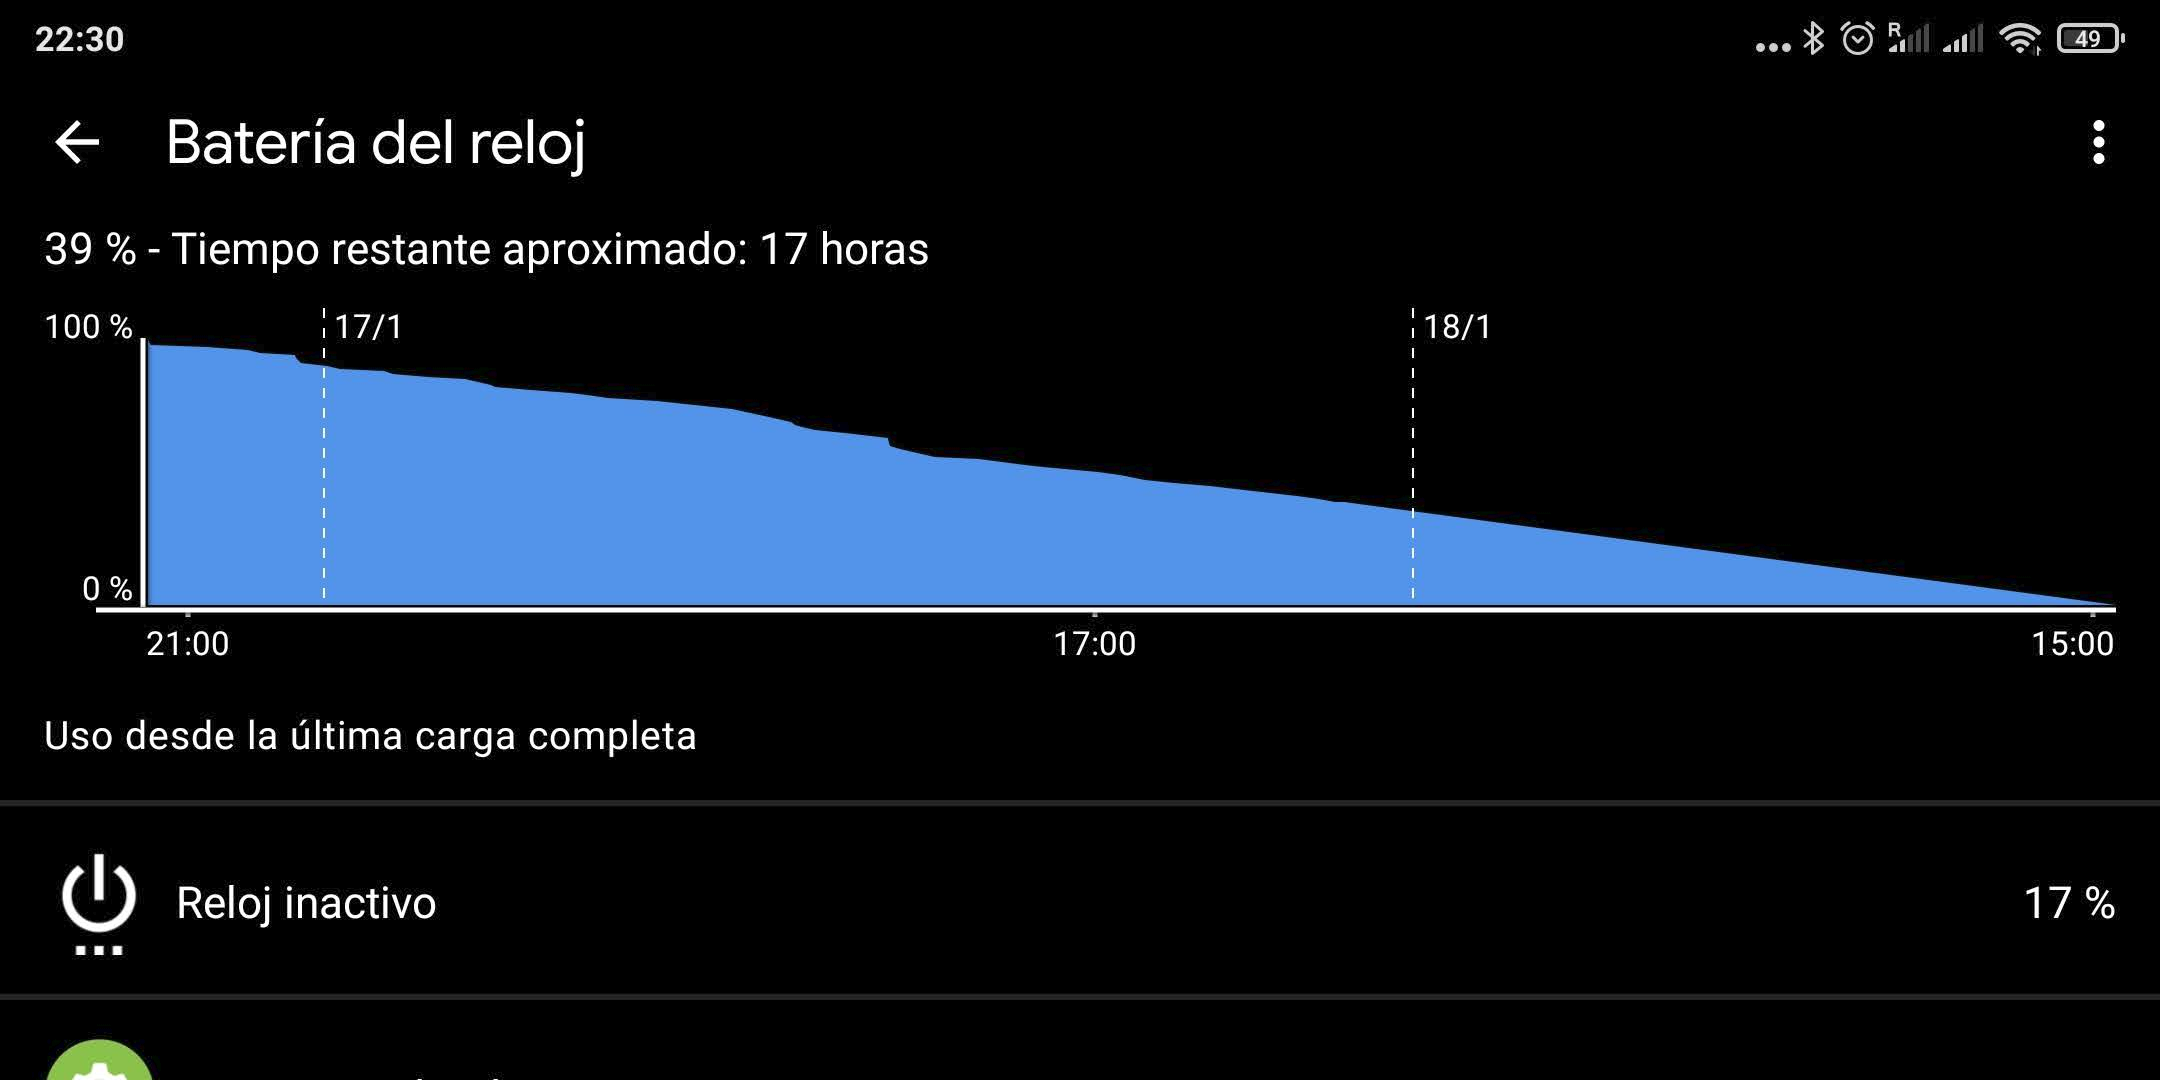
\includegraphics[width=0.95\columnwidth]{img/appBatt.png}
  \caption{\label{fig:ifell:bat} Estimación de autonomía del sistema llevable ejecutando \ifell/}
\end{figure}

\section{DISCUSIÓN O ANÁLISIS DE RESULTADOS}

El primer hito de este trabajo es demostrar que los modelos híbridos permiten integrar en un dispositivo llevable un sistema autónomo de detección de caídas usando técnicas de aprendizaje automático y mantener el consumo de batería al mínimo. 

El modelo de detección de caídas basado en aprendizaje no supervisado y detección de anomalías, sin ser el más adecuado para la tarea, ha demostrado sus capacidades. Especialmente prometedor es el sistema basado en predicción, pues aunque en este estudio ha dado resultados más pobres que su hermano de reconstrucción de la señal de entrada, sus aplicaciones entrenado con un conjunto adecuado podrían en ciertas circunstancias lanzar una alerta segundos antes de la propia caída con el objetivo de prevenirla. 
Sin embargo en cuanto a su capacidad como clasificador se encuentra lejos de la de otros trabajos basados en otras técnicas. El 82,2\% de exactitud ponderada está 15 puntos por debajo de sus hermanos basados en aprendizaje automático. Además, hay que reducir la sensibilidad por debajo del 99\%. Dado que una caída es un evento crítico, debemos forzar el uso de una sensibilidad lo más alta posible, en ese caso la especificidad de \ifell/ cae hasta el 58,5\%, que si bien es baja, mejora considerablemente el resultado del modelo analítico de Bourke. 

Achacamos los resultados del clasificador a la baja correlación de la señal aceleración media en la muñeca pues obliga a al codificador/decodificador o bien a sobreadaptarse al conjunto de entrenamiento (como se aprecia en las curvas del RMSE durante el entrenamiento) o bien lograr una generalización que cubra parte del espacio de las anomalías o caídas y ser por tanto capaz de reconstruirlas con la misma precisión que de una actividad normal se tratara. No obstante confiamos en la buena capacidad del codificador RNN para la extracción de características que puedan servir a la posterior discriminación de las caídas. 


\section{CONCLUSIONES}
Este trabajo presenta un sistema de detección de caídas totalmente autónomo con especial énfasis en ser práctico para el usuario final. Para conseguir dichas metas abordamos 3 pilares u objetivos principales:

\begin{itemize}
	\item Ofrecer una solución realizable, útil y que no suponga una traba al usuario final. Orientado especialmente a personas mayores.
	\item Implementar un sistema de detección eficiente en consumo de recursos.
	\item Aportar un sistema de detección de caídas que sepa generalizar y detectar todo tipo de ellas.
\end{itemize}

Ofrecemos una solución basada en un algoritmo de detección mediante de dos etapas o híbrido para aunar la frugalidad de los algoritmos analíticos con la potencia de los algoritmos basados en técnicas de aprendizaje automático. Presentamos un novedoso modelo de detección de caídas basado en la arquitectura RNN codificador/decodificador para la extracción de características de la señal del módulo de la aceleración y su reconstrucción que mediante la arquitectura híbrida del algoritmo permite mejorar hasta en un 41\% la especificidad del modelo de Bourke a igual sensibilidad (99\%) mientras mantenemos una autonomía superior a 24 horas de funcionamiento de la que no hay precedente en la literatura de sistemas de detección mediante aprendizaje automático. Demostrando así que el uso de RNN para la extracción de características es un sistema competente incluso con capturas de señal muy ruidosas. Con el objetivo de ofrecer un producto práctico, familiar y de fácil uso para personas mayores integramos el desarrollo en un reloj inteligente o \textit{smartwatch}.

% TODO cita Liu2020? sobre la duraciónd e la batería, 

%TODO alguna de las citas sobre la muñeca es mala idea
Elegir un reloj  como plataforma para la implementación obliga a tomar las medidas de los sensores desde una extremidad con alta movilidad y baja congruencia con el cuerpo reduce la calidad de la fuente de datos lastrando los resultados del sistema. De cara a posibles evoluciones sería deseable incorporar nuevos sensores inerciales y de constantes vitales para enriquecer estas fuentes. Así mismo sería recomendable sustituir la etapa del decodificador de las características por un sistema de clústering o clasificación como \textit{k-means}. Alternativamente, si la plataforma lo soporta se podría estudiar el suplantar ya sea el decodificador como directamente el modelo completo por el módulo discriminador de una \textit{GAN}.

\appendix
\section{APÉNDICES}

\bibliographystyle{unsrt}
\bibliography{tfm}

\end{document}
